% NOVA paper — IEEE conference format.
% Build:  latexmk -pdf main.tex      (MiKTeX / TeX Live; also works on Overleaf after uploading ../experiments/paper)
% Tables and figures come from experiments/analysis/paper_results.py; re-run it after new experiments.
\documentclass[conference]{IEEEtran}
\IEEEoverridecommandlockouts

\usepackage[utf8]{inputenc}
\usepackage[T1]{fontenc}
\usepackage{amsmath,amssymb}
\usepackage{graphicx}
\usepackage{booktabs}
\usepackage{catchfile}
\usepackage{multirow}
\usepackage{xcolor}
\usepackage{algorithm}
\usepackage{algpseudocode}
\usepackage[hidelinks]{hyperref}
\usepackage[capitalise,noabbrev]{cleveref}

\graphicspath{{../experiments/paper/}}
\newcommand{\results}[1]{../experiments/paper/#1}
% Placeholder for numbers that are filled in once all runs finish. Remove before submission.
\newcommand{\TBD}[1]{\textcolor{red}{[#1]}}
\newcommand{\nova}{\textsc{Nova}}
\newcommand{\unk}{\textsc{unknown}}

\begin{document}

\title{\nova: Novelty-aware, Open-world, Validated Adaptation for Network Intrusion Detection under Delayed and Scarce Labels}

\author{
\IEEEauthorblockN{\TBD{Author Name}}
\IEEEauthorblockA{\TBD{Affiliation}\\ \TBD{email}}
}

\maketitle

\begin{abstract}
Machine-learning network intrusion detectors are trained once and then meet traffic that drifts and attack
classes that did not exist at training time, while analysts can label only a small and late fraction of the flows.
Published approaches address these problems one at a time: drift adaptation for binary detectors, open-set
rejection on static splits, or active learning without label delay. We study them together on chronological
replays of CIC-IDS2017, CSE-CIC-IDS2018 and UNSW-NB15 with a fixed label budget and a one-window label delay,
and we propose \nova{}, an adaptation loop that (i)~rejects flows that are far from every known class with a
class-conditional $k$-nearest-neighbour detector, (ii)~spends the label budget on novel and diverse traffic modes,
(iii)~propagates analyst labels to agreeing neighbours, (iv)~keeps rare attack classes in a class-balanced memory,
and (v)~deploys a model update, or a rollback, only after it passes a hold-out and a forgetting check.
Under one protocol and the same labelling cost, we compare \nova{} with eight methods, including
re-implementations of INSOMNIA, NetGuard's density-aware selection, uncertainty sampling and class-balanced
replay. On CIC-IDS2017 \nova{} reaches an open-world macro-F1 of 0.768 (best baseline 0.756) and a binary
detection F1 of 0.854 at a 2.8\% false-positive rate (best baseline 4.5\%); with 1\% of the flows labelled its
lead grows to nine points (0.651 against 0.561). On UNSW-NB15, where stale rejection thresholds pull every other
adaptive method below the never-updated model, \nova{} is the only one above it (0.509 against 0.499). On
CSE-CIC-IDS2018 it ties the strongest baseline (0.722) with 35\% fewer false positives and five times less
forgetting.
We release the evaluation console, configurations and per-flow predictions.
\end{abstract}

\begin{IEEEkeywords}
network intrusion detection, concept drift, open-set recognition, active learning, continual learning
\end{IEEEkeywords}

\section{Introduction}
\label{sec:intro}

Flow-based intrusion detectors routinely report accuracies above 99\% on benchmarks such as
CIC-IDS2017~\cite{sharafaldin2018}, mostly with random train/test splits in which flows of one attack session
fall on both sides. Network traffic is time-dependent, and estimates from a chronological split differ from those
of a random split~\cite{nismara2026temporal}; careful sequence evaluations find that the protocol matters far more
than the model architecture~\cite{moczkodan2026transformers}.

A deployed detector faces three further conditions. \emph{New attack classes} appear after training, and a
closed-set model assigns them to a known class, most often benign. \emph{Labels are scarce}: an analyst inspects
a small fraction of the flows. \emph{Labels are late}: ground truth arrives after the decisions were made. In
addition, every model update is a deployment, and a bad one degrades detection silently. Prior work handles
these conditions one at a time (\cref{sec:related}).

We study them together and propose \nova{} (Novelty-aware, Open-world, Validated Adaptation). Our
contributions are:
\begin{enumerate}
  \item a protocol for drift-aware open-world NIDS: chronological replay in windows, a label oracle that enforces
        one budget and delay for every method, and metrics that stay comparable when methods learn different
        classes (\cref{sec:problem});
  \item \nova{}, which combines class-conditional $k$-NN rejection with per-class recalibration, a
        novelty-weighted, cluster-diverse query, agreement-checked label propagation, a class-balanced memory
        and a guarded deployment with rollback (\cref{sec:method});
  \item a comparison with eight methods, including four re-implemented from the literature, on three datasets,
        with an ablation of every component (\cref{sec:setup,sec:results}). Code, configurations and per-flow
        predictions will be released with the final version.
\end{enumerate}

\section{Related Work}
\label{sec:related}

\textbf{Evaluation methodology and datasets.}
TESSERACT~\cite{pendlebury2019tesseract} showed that spatial and temporal bias inflate malware-detection results
and introduced time-consistent splits and the area-under-time (AUT) metric. Arp et al.~\cite{arp2022dos} found
ten such pitfalls across 30 top-venue security papers. For NIDS data specifically, Engelen et
al.~\cite{engelen2021troubleshooting}, Lanvin et al.~\cite{lanvin2022errors} and Liu et al.~\cite{liu2022error}
document labelling and feature-extraction errors in CIC-IDS2017 and CSE-CIC-IDS2018. We follow their advice:
chronological replay, preprocessing fitted on the training period only, multiple seeds, and baselines run
under our protocol rather than numbers copied across papers.

\textbf{Drift detection and rejection.}
Transcend~\cite{jordaney2017transcend} and its successor~\cite{barbero2022transcending} attach conformal
credibility to any classifier and reject low-credibility predictions. CADE~\cite{yang2021cade} learns a
contrastive embedding and flags samples far from every class centroid. OWAD~\cite{han2023owad} calibrates
anomaly-detector outputs, tests for normality shift and selects the samples that explain it. These methods
detect or explain drift; \nova{} also decides what to label and when an update may be deployed.

\textbf{Adaptive and continual NIDS.}
INSOMNIA~\cite{andresini2021insomnia} retrains a detector on pseudo-labels from a nearest-centroid estimator,
without analyst labels after deployment. ENIDrift~\cite{wang2022enidrift} maintains an ensemble of
sub-classifiers over incremental packet embeddings. AOC-IDS~\cite{zhang2024aoc} fine-tunes a contrastive
autoencoder on Gaussian-fit pseudo-labels; SSF~\cite{zhang2025ssf} adds drift-triggered strategic sample
selection and forgetting; Mousavipour et al.~\cite{mousavipour2025shift} add distribution-level shift
explanation and relational distillation. SOUL~\cite{amalapuram2024soul} and Amalapuram et
al.~\cite{amalapuram2023augmented} study continual learning with replay memories, including class-balanced
reservoirs~\cite{chrysakis2020online}. Almost all of these are binary detectors; none rejects unknown traffic
per flow while also modelling label delay.

\textbf{Active learning under drift.}
Chen et al.~\cite{chen2023continuous} combine hierarchical contrastive learning with a similarity-based
uncertainty score for monthly Android-malware relabelling. NetGuard~\cite{gupta2025netguard} selects flows by
a density ratio between new and labelled traffic and synthesises minority attacks. CLUE~\cite{prabhu2021clue}
clusters uncertainty-weighted embeddings to pick uncertain and diverse samples. \nova{}'s query belongs to this
family, but weights clusters by an open-world novelty score and runs every window under a label delay.

\textbf{Open-set recognition for NIDS.}
EVT/OpenMax-style detectors~\cite{zhang2020osr} estimate an unknown-class probability. Corsini and
Yang~\cite{corsini2023ood} compare six out-of-distribution detectors on CIC data and find $k$-NN distance on
embeddings the strongest single detector, in line with deep $k$-NN results in vision~\cite{sun2022knn}.
\nova{} uses a class-conditional variant and recalibrates it as new classes are learned.

\section{Problem Setting and Protocol}
\label{sec:problem}

\textbf{Stream.} Flows $(x_t, y_t)$ arrive in timestamp order, where $x_t \in \mathbb{R}^d$ are flow features and
$y_t$ is one of a class set that grows over time. A model is trained on an initial period whose classes $C_0$
are known. The rest of the stream is processed in windows $W_1, W_2, \dots$ of $n$ flows each.

\textbf{Decisions.} For each flow the deployed model outputs a known class or \unk{}. \unk{} means
``unfamiliar to this model, send to an analyst''; it is neither an alarm nor a statement that the flow is
malicious.

\textbf{Labels.} After predicting $W_w$, a method may request ground truth for at most $B\cdot n$ flows of
$W_w$ (budget $B$). The labels arrive at window $w+\delta$ (delay $\delta$). A label oracle is the only
path to ground truth: it enforces the budget and delay and counts every label it hands out. Methods that do
not choose which flows to label receive a uniform random sample of the budget.

\textbf{Deployment.} A method may replace the deployed model after any window; the new model affects only later
windows. There is no look-ahead: preprocessing statistics are fitted on the training period only, and the last
fraction of the training period is held out as a fixed reference set used to measure forgetting. The reference
set keeps only classes that occur in the fitted part of the training period: a class that first appears in the
reference period (SSH-Patator in CIC-IDS2017) was never learned, and keeping it would turn ``forgetting'' into a
measure of unknown-attack detection.

\textbf{Metrics.} Let $\mathcal{C}$ be the set of all true classes in the stream. Standard open-set macro-F1 maps
a flow to \unk{} when its class is unknown to the model that scored it, so two methods that learn different
classes are scored on different label sets. We therefore report
\begin{itemize}
\item \emph{open-world macro-F1} (OW-F1): macro-F1 over the fixed set $\mathcal{C}$, where a flow counts as
      correct if the decision is its true class, or if its class is unknown to the deployed model and the decision
      is \unk{};
\item \emph{AUT(OW-F1)}: the area under the per-window OW-F1 curve, normalised to $[0,1]$~\cite{pendlebury2019tesseract};
\item binary \emph{detection} F1, recall and false-positive rate, where a flow is flagged when the decision is not
      benign (an attack class or \unk{}; both reach an analyst), for comparison with binary NIDS work;
\item \emph{unknown AUROC}: how well the open-world score separates flows of classes unknown to the deployed
      model from known-class flows;
\item \emph{maximum forgetting}: the largest drop of macro-F1 on the reference set below its running maximum;
\item labels used and training time.
\end{itemize}

\section{\nova{}}
\label{sec:method}

\nova{} wraps any probabilistic classifier $f$ (gradient-boosted trees in our experiments). It keeps a training
memory $M$, a calibration store $Q$ of held-out analyst labels, and the previously deployed model.
\Cref{alg:nova} gives the per-window loop; the components are described below.

\begin{algorithm}[t]
\caption{\nova{}, one window $W_w$}
\label{alg:nova}
\begin{algorithmic}[1]
\State predict $W_w$ with $f$; compute unknown scores $s(x)$ \Comment{\cref{sec:unknown}}
\State request labels for $\textsc{Query}(W_w, s, B n)$ \Comment{arrive at $w{+}\delta$; \cref{sec:query}}
\State $L \gets$ labels that arrived now
\If{$f$ was just deployed \textbf{and} $f_{\text{prev}}$ beats $f$ on $L$ by $>\rho$ \textbf{and} the reference check passes}
   \State roll back to $f_{\text{prev}}$ \Comment{\cref{sec:guard}}
\EndIf
\State $H \gets$ stratified hold-out of $L$; \ $T \gets L\setminus H$
\State $P \gets \textsc{Propagate}(T)$ \Comment{\cref{sec:prop}}
\State $f' \gets \textsc{Train}(M \cup T \cup P)$, newest labels weighted $\omega$; calibrate on reference $\cup\, Q$
\If{$\mathrm{F1}_H(f') \ge \mathrm{F1}_H(f)$ \textbf{and} $\mathrm{F1}_{\text{ref}}(f) - \mathrm{F1}_{\text{ref}}(f') \le \epsilon$}
   \State deploy $f'$
\EndIf
\State $M \gets \textsc{CBRS}(M, T \cup P)$; move $H$ to $Q$ (classes already in $M$) or to $M$
\end{algorithmic}
\end{algorithm}

\subsection{Open-world scoring}
\label{sec:unknown}
For a flow $x$ with predicted class $c = \arg\max_k p_k(x)$, \nova{} computes two scores, each scaled so that its
threshold is 1:
\begin{align}
s_{\text{msp}}(x) &= \frac{1 - p_c(x)}{1 - \tau^{\text{msp}}_c}, &
s_{\text{knn}}(x) &= \frac{d_k\!\left(x, \mathcal{B}_c\right)}{\tau^{\text{knn}}_c},
\end{align}
where $d_k(x,\mathcal{B}_c)$ is the distance to the $k$-th nearest training flow of class $c$ in a per-class bank
$\mathcal{B}_c$. The thresholds are per class: $\tau^{\text{msp}}_c$ is a low quantile (2\%) of the confidence of
held-out flows predicted as $c$, and $\tau^{\text{knn}}_c$ a high quantile (99\%) of $d_k$ on held-out flows of $c$.
The unknown score is $s(x) = \max(s_{\text{msp}}, s_{\text{knn}})$ and the decision is \unk{} iff $s(x) > 1$.
Conditioning the neighbour search on the predicted class follows multi-modal classes such as benign traffic, which
a single centroid~\cite{yang2021cade} cannot. Thresholds are recomputed for every model version on the reference set
plus the calibration store, so classes learned during deployment receive their own thresholds instead of the
strictest fallback.

\subsection{Query}
\label{sec:query}
Of the budget $Bn$, a share $\rho_u$ is drawn uniformly to keep an unbiased view of benign drift. The rest is
spread over $K$ $k$-means clusters of the window: each cluster $j$ receives at least one label and a quota
proportional to $\sqrt{|j|}\,\bigl(0.1 + \bar{s}_j\bigr)$, where $\bar{s}_j$ is the mean clipped unknown score of
the cluster; inside a cluster, the highest-scoring flows are chosen. Square-root size damping keeps large drifting
benign modes covered while emerging attack modes, which are both novel and compact, receive many labels.

\subsection{Label propagation}
\label{sec:prop}
An unlabelled flow $u$ of the same window takes class $c$ when its $\min(k_p, n_c)$ nearest labelled flows all have
class $c$ and its nearest distance is within the radius of $c$ (the 90th percentile of nearest-same-class distances
among the labels of $c$). At most $r$ propagated labels are kept per analyst label of $c$. Unlike
self-training~\cite{andresini2021insomnia,zhang2024aoc}, propagation is anchored on analyst labels and never
creates a class.

\subsection{Memory}
\label{sec:memory}
The training memory is a class-balancing reservoir~\cite{chrysakis2020online}: once full, a sample of a class that is
not the largest evicts a random sample of the largest class. ``Largest'' compares size divided by a class weight,
and benign traffic receives weight $\beta$: it is multi-modal, and starving it raises false alarms.

\subsection{Deployment guard and rollback}
\label{sec:guard}
A candidate is deployed only if it is at least as good as the current model on the held-out slice $H$ of the newest
analyst labels and loses at most $\epsilon$ macro-F1 on the reference set. Both comparisons use the open-world
credit of \cref{sec:problem}, so models that know different classes are compared on the same task, and ignore
classes with fewer than $m$ labels in the compared slice. A rollback is itself a deployment and must pass the same
reference check; without it, a rollback to an early model can undo what the stream has taught.

\section{Experimental Setup}
\label{sec:setup}

\textbf{Datasets.} \Cref{tab:datasets} summarises the three datasets. All are replayed in timestamp order.
From each we take 400{,}000 flows evenly spaced over time (deterministic); the first 30\% form the training
period (its last 20\% is the reference set) and the remaining 280{,}000 flows form 70 windows of 4{,}000 flows.
CIC-IDS2017~\cite{sharafaldin2018} uses the \texttt{TrafficLabelling} CSVs, whose timestamps lack AM/PM; we
restore afternoon times. The fitted part of its training period (Monday and Tuesday morning) contains only
benign traffic and FTP-Patator, so twelve attack classes are new. For CSE-CIC-IDS2018 we use the ``Processed Traffic Data for ML''
CSVs, thinned to one row in eight per file before sampling; seven attack classes are known at training time and
seven appear later. In UNSW-NB15~\cite{moustafa2015unsw} every class already occurs in the first capture day, so,
as is common in open-set NIDS work, we remove DoS, Reconnaissance, Shellcode and Worms from the training
period; they appear in the stream as unknown attacks.

\begin{table}[t]
\centering
\caption{Datasets (after replay sampling: 400k flows, 70 windows).}
\label{tab:datasets}
\resizebox{\columnwidth}{!}{%
\begin{tabular}{@{}lccc@{}}
\toprule
 & CIC-IDS2017 & CSE-CIC-IDS2018 & UNSW-NB15 \\
\midrule
Source flows & 2.83\,M & 16.2\,M & 2.54\,M \\
Days covered & 5 & 10 & 2 \\
Classes (incl.\ benign) & 15 & 15 & 10 \\
Attack classes in training & 1 & 7 & 5 \\
New in stream & 12 & 7 & 4 (held out) \\
\bottomrule
\end{tabular}}
\end{table}

\textbf{Labels.} Budget $B = 10\%$ (main) and $1\%$ of each window, delay $\delta = 1$ window. Every method that
uses labels gets exactly the same number; INSOMNIA uses none by design.

\textbf{Model.} All methods use the same classifier: scikit-learn histogram gradient boosting (150 iterations,
L2 regularisation 1.0); classes with fewer than five labelled flows are left out of training and stay \unk{}.
All methods also use the same open-world detector (maximum softmax probability and class-conditional $k$-NN),
except in the detector ablation, so differences come from the adaptation strategy.

\textbf{Baselines.} \emph{Static} (never updated); \emph{periodic retrain} (from scratch every five windows on
the training data and the last five labelled windows); \emph{continual replay} (uniform reservoir memory, retrain
whenever labels arrive); \emph{guarded selective} (drift- or novelty-triggered retrain with a hold-out guard and
rollback). Re-implemented under our protocol: \emph{uncertainty sampling} (least-confidence query, INSOMNIA's
``US + oracle'' upper bound~\cite{andresini2021insomnia}); \emph{INSOMNIA}~\cite{andresini2021insomnia}
(least-confident 50\% of each window labelled by a nearest-centroid estimator, no analyst labels);
\emph{NetGuard PS}~\cite{gupta2025netguard} (density-ratio query with two diagonal Gaussian mixtures; the
generative augmentation is not reproduced); and \emph{CBRS replay}~\cite{chrysakis2020online,amalapuram2023augmented}
(class-balancing reservoir memory). All replay memories hold 20{,}000 flows.

\textbf{Development and held-out data.} All design decisions, including the ablation, were made on
CIC-IDS2017. CSE-CIC-IDS2018 and UNSW-NB15 were used for no design decision (we only checked their class
composition with one run of the static model, which led to the UNSW-NB15 hold-out above). Both are
evaluated only with the configuration frozen on CIC-IDS2017.

\textbf{\nova{} hyper-parameters} were fixed from design arguments and two development runs, then frozen:
uniform share $\rho_u = 0.2$, $K = 24$ clusters, $k_p = 5$, $r = 5$, benign weight $\beta = 4$, 25\% hold-out,
calibration store of 200 flows per class (after 50 in memory), minimum support $m = 5$, $\epsilon = 0.05$,
rollback margin $0.05$, recency weight $\omega = 2$, $k = 10$ with 3{,}000 flows per class bank.

\textbf{Runs.} Three seeds per configuration (the seed changes model initialisation, label sampling and
clustering, not the data); we report mean $\pm$ standard deviation. To compare two methods we take the
per-window difference of their seed-averaged OW-F1 (or FPR) and report its mean with a 95\% moving-block bootstrap
interval~\cite{kunsch1989jackknife} (blocks of five windows, 10{,}000 resamples), which respects the autocorrelation of consecutive windows;
we call a difference significant only if the interval excludes zero. Neural variants use PyTorch 2.14.1 with CUDA
13.0 on an RTX 3060; everything else runs on a 16-core CPU.

\section{Results}
\label{sec:results}

% Rows are generated by experiments/analysis/paper_results.py (<group>_paper.tex).
\newcommand{\resulttable}[3]{%
\begin{table}[t]
\centering
\caption{#2 Mean$_{\pm\text{std}}$ over three seeds; best mean in bold. FPR in \%.}
\label{#3}
\footnotesize
\setlength{\tabcolsep}{3pt}
\IfFileExists{\results{#1}}{%
\CatchFileDef{\resultrows}{\results{#1}}{}% \input is not usable inside a tabular
\resizebox{\columnwidth}{!}{%
\begin{tabular}{@{}lcccccc@{}}
\toprule
Method & OW-F1 & AUT & Det-F1 & FPR & U-AUROC & Forget.\\
\midrule
\resultrows
\bottomrule
\end{tabular}}}{\TBD{\detokenize{#1} not generated yet}}
\end{table}}

\subsection{Main comparison}
\resulttable{CIC17_main_b010_paper.tex}{CIC-IDS2017, label budget 10\%, delay 1 window.}{tab:cic17}
\resulttable{IDS18_main_b010_paper.tex}{CSE-CIC-IDS2018, label budget 10\%, delay 1 window.}{tab:ids18}
\resulttable{UNSW_main_b010_paper.tex}{UNSW-NB15 (four classes held out of training), label budget 10\%.}{tab:unsw}

\textbf{CIC-IDS2017} (\cref{tab:cic17}). \nova{} has the highest OW-F1 (0.768) and AUT (0.858), but its lead
over CBRS replay (0.756, 0.838) is within the bootstrap uncertainty (per-window difference $+2.0$ points, 95\% CI
$[-0.5, +4.3]$). It is significantly ahead of every other method (by 6.8 to 22.8 points). CBRS detects slightly
more attacks (detection F1 0.861 against 0.854), but \nova{} flags significantly fewer benign flows (4.5\% against
2.8\% pooled; per-window difference $-4.0$, CI $[-8.8, -0.5]$): it sends 38\% fewer benign flows to the analyst.

\begin{figure}[t]
\centering
\IfFileExists{\results{fig_ow_f1_over_time_UNSW_col.pdf}}{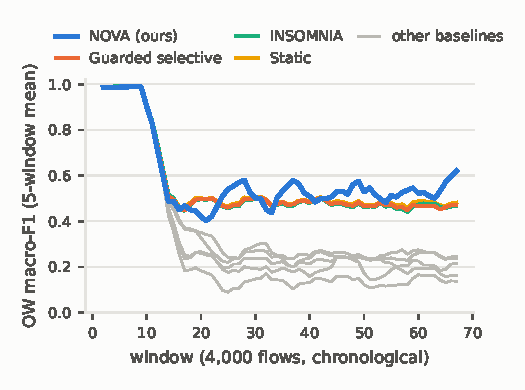
\includegraphics[width=\columnwidth]{fig_ow_f1_over_time_UNSW_col.pdf}}{\TBD{figure}}
\caption{OW macro-F1 per window on UNSW-NB15 (mean of three seeds, 5-window moving average). Replay-based
baselines (grey) fall below the static model.}
\label{fig:time-unsw}
\end{figure}

\textbf{CSE-CIC-IDS2018} (\cref{tab:ids18}). \nova{} and CBRS replay tie on OW-F1 (0.722) and AUT (0.869;
difference CI $[-1.9, +1.9]$). \nova{} has the higher detection F1 (0.815 against 0.788), a significantly lower
false-positive rate (3.1\% against 4.8\%; CI $[-6.9, -0.4]$) and five times less forgetting (0.007 against 0.034).

\textbf{UNSW-NB15} (\cref{tab:unsw}, \cref{fig:time-unsw}). Most adaptive methods end \emph{below} the static
model (0.499); CBRS replay reaches 0.327. They learn Exploits and Fuzzers, but every later flow of these classes is
rejected as \unk{}: the thresholds were calibrated on January traffic, and February flows of the same classes lie
outside them. \nova{} recalibrates learned classes on its calibration store and reaches 0.509 OW-F1 and 0.595
AUT, significantly ahead of every replay-based method ($+19.5$ to $+29.3$ points) and level with the static model
($+2.6$, CI $[-0.1, +4.8]$), with the highest detection F1 (0.860) and lowest false-positive rate (6.6\% against
7.6--19.0\%). On the classes the model knows, \nova{} reaches a macro-F1 of 0.510 against at most 0.165 for any
other method. Without the calibration store, \nova{} drops to 0.418 and zero F1 on Exploits and Fuzzers
(\cref{tab:ablation}), confirming the mechanism.

INSOMNIA's self-training has the highest false-positive rate on both CIC datasets (12.4\%, 25.7\%):
pseudo-label errors on unseen classes are fed back into training.

\Cref{fig:time-cic} shows where the methods differ on CIC-IDS2017. Every method drops when a new attack class
starts. CBRS replay recovers faster from the first DoS attacks (windows 8--12), \nova{} from most later ones,
most visibly in the last ten windows.

\begin{figure*}[t]
\centering
\IfFileExists{\results{fig_ow_f1_over_time_CIC17.pdf}}{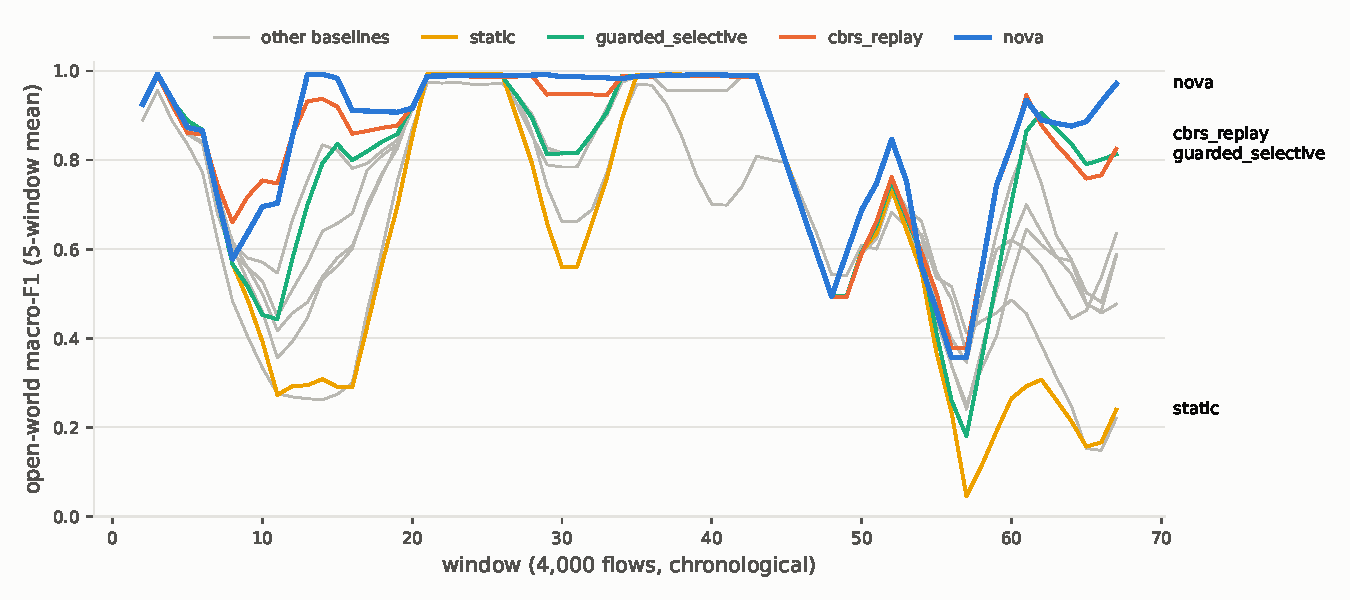
\includegraphics[width=0.8\textwidth]{fig_ow_f1_over_time_CIC17.pdf}}{\TBD{figure}}
\caption{OW macro-F1 per window on CIC-IDS2017 (mean of three seeds, 5-window moving average). \nova{}, the two
strongest baselines and the static model in colour, the other baselines in grey.}
\label{fig:time-cic}
\end{figure*}


\subsection{Label budget}
With 1\% of each window labelled (\cref{tab:budget}), \nova{} leads CBRS replay by 9.0 points on CIC-IDS2017
(per-window CI $[+1.4, +11.6]$) and by 3.4 points on CSE-CIC-IDS2018 (CI $[-0.2, +5.0]$, not significant). On
UNSW-NB15 it trails periodic retraining (0.469 against 0.504). With 40 labels per window, periodic retraining never
collects enough labels of the held-out classes to learn them, so it keeps rejecting them as \unk{}, which the
metric credits in full. Its macro-F1 on the classes the model knows is only 0.154, against 0.383 for \nova{}, which
names 64\% of known attack flows correctly against 7\%. \nova{} learns DoS and Reconnaissance, which overlap with
Exploits, and loses the \unk{} credit; open-world macro-F1 alone cannot separate ``never learned'' from ``learned
imperfectly''. \nova{} also halves the false-positive rate (9.7\% against $\geq$15.7\%).

\begin{table}[t]
\centering
\caption{Label budget 1\%: OW macro-F1 and FPR (\%), mean over three seeds; best per column in bold.}
\label{tab:budget}
\footnotesize
\setlength{\tabcolsep}{3pt}
\IfFileExists{\results{budget_b001_paper.tex}}{%
\CatchFileDef{\budgetrows}{\results{budget_b001_paper.tex}}{}%
\resizebox{\columnwidth}{!}{%
\begin{tabular}{@{}lcccccc@{}}
\toprule
\budgetrows
\bottomrule
\end{tabular}}}{\TBD{budget table not generated yet}}
\end{table}

\subsection{Ablation and detector}
\begin{table}[t]
\centering
\caption{Ablation (budget 10\%): OW-F1 (change in points) and FPR (\%) with one component removed. Mean over
three seeds; full \nova{} over the same seeds. Only CIC-IDS2017 was used for design.}
\label{tab:ablation}
\footnotesize
\setlength{\tabcolsep}{2pt}
\IfFileExists{\results{ablation_all_paper.tex}}{%
\CatchFileDef{\ablrows}{\results{ablation_all_paper.tex}}{}%
\resizebox{\columnwidth}{!}{%
\begin{tabular}{@{}lcccccc@{}}
\toprule
 & \multicolumn{2}{c}{CIC-IDS2017} & \multicolumn{2}{c}{CSE-CIC-IDS2018} & \multicolumn{2}{c}{UNSW-NB15} \\
Variant & OW-F1 & FPR & OW-F1 & FPR & OW-F1 & FPR \\
\midrule
\ablrows
\bottomrule
\end{tabular}}}{\TBD{ablation table not generated yet}}
\end{table}

On CIC-IDS2017 every removal lowers OW-F1 (\cref{tab:ablation}), most for the guard ($-5.6$, in every seed). The
loss is concentrated in XSS and Bot: without the guard, models that name XSS flows Brute Force are deployed, whereas
with it XSS stays \unk{} and receives full open-world credit. Per window, no single removal is significant on
CIC-IDS2017. On UNSW-NB15 the guard and the calibration store are essential ($-22.1$, $-9.1$); both variants lose
Exploits and Fuzzers. On CSE-CIC-IDS2018 the stream-level changes have inconsistent signs across seeds, because four
of its classes have only 2 to 33 flows. Per window, only the query and propagation help significantly there
(block-bootstrap CIs $[-3.1, -0.3]$ and $[-3.6, -0.5]$). Replacing the class-conditional $k$-NN detector by
distance to the nearest class centroid lowers OW-F1 from 0.768 to 0.712 for \nova{} and from 0.311 to 0.178 for
the static model, which then labels almost every attack benign: one centroid cannot follow multi-modal benign
traffic.

\textbf{Neural classifier.} With an MLP instead of gradient boosting on CIC-IDS2017, \nova{} keeps the lowest
false-positive rate (3.3\% against 4.7\%), the higher detection F1 and an equal AUT, but its OW-F1 is lower than
CBRS replay's (0.622 against 0.711), mainly on two short-lived web attacks. We do not claim that its accuracy
advantage carries over to neural classifiers.

\section{Discussion and Threats to Validity}
\label{sec:discussion}

\textbf{Review load.} Most benign flows flagged by any method are \unk{} decisions set by shared quantiles. Even
2.8\% means about 28{,}000 reviews per million benign flows (the base-rate fallacy~\cite{arp2022dos}).

\textbf{Data limits.} Some CIC-IDS2017 port scans are feature-identical to benign flows, Brute Force and XSS are
barely separable~\cite{engelen2021troubleshooting}, and SSH-Patator and slowloris end before any label can arrive
under a one-window delay. Several CSE-CIC-IDS2018 day files are truncated in the published CSVs. The datasets span
two to ten days, so long-term benign drift is under-represented.

\textbf{Protocol.} Baselines are re-implemented in one multi-class framework with the same classifier and
labelling cost; NetGuard's generative augmentation is not reproduced. The oracle is error-free with a fixed delay.
Hyper-parameters were frozen on CIC-IDS2017 and reused unchanged.

\section{Conclusion}
\label{sec:conclusion}

Evaluated under realistic conditions---chronological replay, attack classes that appear after training, and a
small, delayed labelling budget---intrusion detectors that are trained once collapse, and simple retraining
schemes forget or flood analysts with reviews. \nova{} combines class-conditional open-world rejection, a
novelty-weighted and diverse query, conservative label propagation, a class-balanced memory and a guarded
deployment loop. At a 10\% budget it is the best or tied-best method on open-world macro-F1 on all three
datasets and has the lowest false-positive rate on all three. At a 1\% budget it leads on both CIC datasets
(by 9.0 and 3.4 points). On UNSW-NB15 at 1\% it trails methods that never learn the new classes and keep
rejecting them, while still halving the false-positive rate. Its
accuracy lead did not carry over to an MLP classifier, and short-lived attacks that look like benign traffic
remain undetected by every method we tried, including a meta-learned embedding. Both are open problems for
future work. All runs,
configurations and per-flow predictions are released with the SentinelAI console.


\bibliographystyle{IEEEtran}
\bibliography{refs}

\end{document}
